\chapter{Background}
Function merging is a powerful code optimisation technique that reduces redundancy by combining similar or identical functions within a program. At its core, function merging involves identifying functions with similar structures and semantics and generating a merged function that uses decision points and parameters to distinguish between the behaviours where the original functions diverge.

\section{The LLVM Compiler} \label{Background:LLVM}
LLVM is an open-source compiler infrastructure project widely used in industry and academia that provides a collection of modular and reusable compiler and toolchain technologies \cite{LLVMMainPage}. 

This project is built upon a state-of-the-art (SOTA) implementation of function merging, F3M \cite{F3M:FastFocusedFunctionMerging},  which was implemented in LLVM. The modular pass-based architecture of LLVM (section \ref{LLVM:Passes}) makes it ideal for integrating new optimisations into the pipeline without too much complexity. Additionally, LLVM is widely adopted across industry and academia, with support for many high-level languages and target architectures, ensuring that our optimisation can have a broad practical impact.

\subsection{LLVM Architecture}
At its core, the LLVM compiler employs a three-phase design. The \textbf{front-end} translates the source code into LLVM Intermediate Representation (LLVM IR), the \textbf{middle-end} performs various transformations and optimisations on the IR, and the \textbf{back-end} generates the machine code for specific target architectures from the IR.

This modular design reduces the implementation effort compared to directly porting each language to each target architecture and it also allows LLVM to support multiple programming languages across multiple target architectures while sharing the middle optimisation layer.

\subsection{LLVM IR} \label{LLVM:IR} \label{LLVM:Bitcode}
LLVM IR serves as a central data structure throughout the compilation process. It is a language-independent, low-level representation designed to support program analysis and transformation. The LLVM IR comes in three flavours: a human-readable assembly-like text format, an in-memory data structure used by compilers, and a dense bitcode format for disk storage \cite{LLVMIR}. 

LLVM IR uses a static single assignment (SSA) form, where each variable is assigned exactly once, making data flow analysis more straightforward. The IR represents programs as a collection of functions, with each function containing basic blocks connected by control flow graphs. Each basic block consists of a sequence of instructions that execute sequentially.

\subsection{LLVM Passes} \label{LLVM:Passes}
LLVM's optimisation framework operates on the IR through a series of passes which analyse or transform the program in steps. Passes are split into three types, the analysis passes which gather information to be used by other passes or the debugger, the transform passes which modify the program in some way and the utility passes which encompass any passes that do not fit into the first two categories \cite{LLVMPasses}. 

The function merging pass described in this paper is located in the middle-end of LLVM, operating on the IR during link time optimisation (LTO). LTO provides the compiler with global visibility and access to all functions across the program, substantially increasing opportunities for identifying and combining similar code by increasing the pool of function candidates \cite{FunctionMergingSequenceAlignment}.

% \section{Compiler}
% Compilers serve as translators that convert high-level programming languages into machine-executable code. Their goal is to produce the most efficient executable code where possible while still preserving semantic correctness. Modern compilers work by performing numerous analyses and transformations to improve the code quality.

% The compilation process can be broadly split into three stages, the front-end, the middle-end and the back-end. The front-end is responsible for lexical analysis, parsing, and semantic analysis to convert source code into an intermediate representation (IR). The IR serves as a language and target independent abstraction of the program. By using an IR, developers can reduce the work needed to add support for a new source language or target, only the connection to the IR must be implemented rather than a completely new pipeline for every other existing target or source. Next, the middle-end analyses and optimises the IR where possible. Finally, the back-end transforms the optimised IR into target-specific machine code through instruction selection, register allocation, and more.

% In modern compilers, optimisations are organised into passes, each concentrating on one type of optimisation. The function merging pass described in this paper is located in the middle-end, operating on the IR during link time optimisation (LTO). LTO allows the compiler to view and optimise the entire program as a unified whole rather than as isolated modules, allowing optimisations across module boundaries. This whole-program visibility enables optimisations to work across module boundaries that would normally be isolated. For function merging especially, LTO provides access to all functions across the program, substantially increasing opportunities for identifying and combining similar code \cite{FunctionMergingSequenceAlignment}. 

% This project is built upon a state-of-the-art (SOTA) implementation of function merging, F3M \cite{F3M:FastFocusedFunctionMerging},  which was implemented in LLVM, a compiler toolchain. The modular pass-based architecture of LLVM makes it ideal for integrating the project into the pipeline without too much complexity. Additionally, LLVM is widely used across industry and academia, meaning that it has support for many high-level languages and target architectures, ensuring that optimisation can have a broad practical impact.

\section{Existing Function Merging Approaches} \label{Background:RelatedWork}
This chapter will discuss the current function merging technique used in LLVM and the previous state-of-the-art solutions to function merging. Function merging is still an actively researched optimisation in compilers, focussing on the orthogonal problems of identifying functions that merge well and how to merge a specific pair of functions.

\subsection{LLVM Function Merging}
The current LLVM implementation adopts a conservative two-phase approach to function merging, prioritising low compilation overhead over maximising merge opportunities, focussing primarily on merging structurally identical functions through an efficient filtering mechanism. 


\subsubsection{Hashing}
The first phase categorises functions using a lightweight hash-based approach to identify potential candidates quickly. The hash aims to capture the function's structural semantics while maintaining the invariant:

\begin{equation}
F1 == F2 \Rightarrow Hash(F1) == Hash(F2)
\end{equation}

It is, therefore, guaranteed that if two functions are the same, they will hash to the same value. This hash function accounts for function signatures, control flow structure, and instruction opcodes. Only functions producing identical hash values proceed to the next phase for a more detailed comparison.

\subsubsection{Detailed Comparison}
In the second phase, a detailed comparison is applied to functions with matching hash values to verify their structural compatibility for merging. This process begins by checking the functions' attributes, return types and parameter types to ensure type consistency. Then, a comprehensive analysis of the function bodies is conducted. This is done by traversing both functions in parallel using their control-flow graph (CFG), visiting every basic block in the graph, and comparing the instructions inside each basic block. Every instruction in the first function is directly compared to the instruction in the second function in the same position, comparing the instruction opcodes and operand types. When a successful match is identified, LLVM creates a unified function that preserves the behaviour of both original functions \cite{LLVMFuncMergSrc}.

\subsubsection{Limitations}
This existing approach is inherently conservative, primarily targeting functions with nearly identical control flow graphs and instruction sequences \cite{LLVMMergeFunctionsPass}. While it accommodates cases where operand types differ but can be safely bitcasted, this flexibility is quite limited. This conservative stance significantly limits merging opportunities, particularly for functions that contain substantial shared code but differ in specific regions. 

These limitations establish a clear opportunity for more sophisticated merging decision mechanisms that recognise non-obvious structural similarities and better predict optimisation benefits.

% \subsection{Function Merging by Sequence Alignment (FMSA)}
% Rocha et al. introduced a novel technique for code size reduction that adapts sequence alignment algorithms from bioinformatics to merge similar functions \cite{FunctionMergingSequenceAlignment}. This technique attempts to address a limitation of previous methods, either merging almost identical functions or algorithms which struggled to identify feasible functions for merging.

% This approach consists of three stages, function linearisation, sequence alignment and code generation. During linearisation, the functions are transformed by traversing the function's blocks in the control-flow graph (CFG). The basic blocks and labels are then expanded where necessary to produce the linearised function consisting of instructions. 

% Next, the algorithm leverages the Needleman-Wunsch algorithm to align instruction sequences, which was originally developed for identifying similarities between amino acids of proteins. This dynamic programming algorithm assesses two linearised functions to identify regions of similarity by inserting blank objects where necessary to maximise matching between equivalent segments. 

% \begin{figure}[tbh!]
% \centering
% 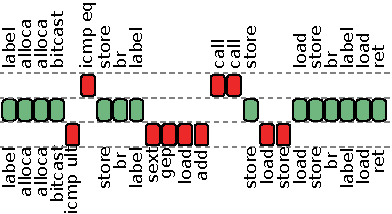
\includegraphics[scale=1]{Figures/FMSA_FunctionSA.pdf}
% \caption{The sequence alignment between two functions, identifying the equivalent segments of code (green in the center) and the non-equivalent ones (red at the sides). Figure and caption taken from \cite{FunctionMergingSequenceAlignment}.}\label{fig:SequenceAlignment2Funcs}
% \end{figure}

% For this to work, criteria were chosen to determine when two instructions are considered to be matching. They are considered matching when they have semantically identical opcodes, equivalent result types and pairwise equivalent operand types. Types are considered equivalent when they can be bitcasted between each other losslessly.

% In the final code generation stage, the aligned instruction segments with equivalent code are merged, while non-equivalent segments are maintained but guarded by a function identifier parameter that is added to the merged function.

% This technique demonstrated amazing results, reducing code size by 25\% on Intel architecture and 30\% on ARM. Approximately 2 times better than the state-of-the-art at the time.

% \subsubsection{Alignment Score} \label{METRIC:AlignmentScore}
% The sequence alignment between two functions is a property that identifies the structural similarity between two functions, serving as a key predictor of function merging profitability. This provides direct insight into how effectively two functions can be merged and is the characteristic our machine learning model aims to predict.
% To quantify this value, the alignment score metric is used, defined as the ratio of the aligned instructions to the union of aligned and unaligned instructions:
% $$Alignment\ Score = \frac{Number\ of\ Aligned\ Instructions}{Total\ Aligned\ and\ Unaligned\ Instructions}$$
% Using figure \ref{fig:SequenceAlignment2Funcs} we can calculate the alignment score as follows:
% $$\frac{No.\ of\ Green\ Nodes}{Total\ No.\ of\ Green\ and\ Red\ Nodes}=\frac{14}{24} = 0.5833$$

% Given that this metric is a ratio, this metric will be a continuous value in the range of [0, 1] inclusive, where 0 represents a completely dissimilar function pair and 1 representing a structurally identical function pair.

% \subsection{HyFM}
% HyFM tries to tackle the inefficiencies of the previous state-of-the-art (SOTA) by introducing multiple optimisations \cite{HyFM:FunctionMergingForFree}. 

% \subsubsection{Basic-Block Granularity} \label{HyFM:BasicBlockGranularity}
% First, HyFM works at the basic-block level instead of function level. While the complexity is still $O(n^2)$ for the Needleman-Wunsch (NW)algorithm, $n$ in the previous SOTA refers to the number of instructions in functions whereas $n$ in HyFM refers to the number of instructions in basic blocks, which is considerably smaller, resulting in a dramatic memory reduction.

% \subsubsection{Fingerprint} \label{HyFM:FingerprintDistance}
% Before performing alignment, HyFM uses fingerprints to efficiently identify similar blocks. Each fingerprint is a fixed-size vector representing the frequency count of each opcode in a block. HyFM pre-computes fingerprints for all basic blocks and uses the Manhattan distance between these fingerprints to pair similar blocks from different functions. This lightweight filtering mechanism helps HyFM quickly focus on promising block pairs before applying the more expensive alignment analysis.


% \subsubsection{Pairwise-Alignment (PA)} \label{HyFM:PairwiseAlignment}
% Additionally, HyFM introduces a new linear-complexity pairwise alignment (PA) strategy that only aligns instructions in corresponding positions, with instructions matching only if they have the same opcode. It has been identified that most basic blocks that would be profitably merged have highly similar structure, making this simpler approach effective for real-world code. Finally, HyFM implements a multi-tiered profitability analysis, allowing it to bail out early from unprofitable and expensive merging attempts. This prevents wasting resources on generating merged code that would ultimately be discarded, contributing to HyFM's speedup compared to the previous SOTA.

% \subsection{F3M: Fast Focused Function Merging}
% \todo {INCLUDE SECTION/IMAGE ON HOW THE FUNCTIONS GET MERGED}


% This project is built on the current state-of-the-art function merging, Fast Focused Function Merging's (F3M) infrastructure. F3M represents the current state-of-the-art in function merging technology to address critical inefficiencies that previously made function merging impractical for large-scale applications. While its predecessor, HyFM, improved function merging by operating at the basic block level \cite{HyFM:FunctionMergingForFree}, F3M introduces fundamental innovations that dramatically reduce compilation time while maintaining or improving code size reduction.

% The technique introduces two key innovations. 

% \subsubsection{Min-Hash Fingerprinting} \label{METRIC: MinHashFingerprint}
% First, F3M employs MinHash-based fingerprinting that better captures the semantic similarity between functions. Each instruction is encoded as a 32-bit integer representing four critical properties: opcode, result type, number of operands, and operand types. These encoded instructions are then grouped into overlapping "shingles" (pairs of consecutive instructions).  Multiple hash functions are then applied to each shingle, with only the minimum hash value across all shingles from each function retained, producing a fixed-length fingerprint vector.

% \begin{figure}[h!]
% \centering
% 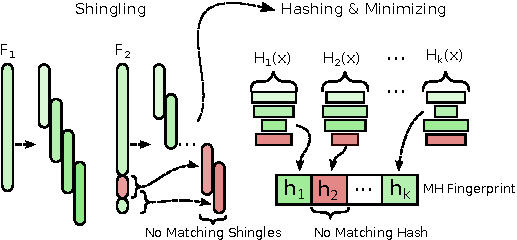
\includegraphics[scale=1]{Figures/F3M_MinHash.pdf}
% \caption{The MinHash algorithm: Textual documents are broken up into overlapping subsequences; Each subsequence is hashed with k different hash functions; For each function, the smallest hash is saved creating a fingerprint of k entries. In this example, two functions differ in only a couple extra instructions inside F2. For F2’s fingerprint, this creates shingles and hashes with no matches in F1, representing the slight difference between them. Figure and caption taken from  \cite{F3M:FastFocusedFunctionMerging}.}\label{fig:testsvg}
% \end{figure}

% \subsubsection{Comparing MinHash Fingerprints} \label{METRIC:MinHashDistance}
% To compare the MinHash fingerprints, the Jaccard Index between two fingerprints is calculated, representing the likelihood of matching instruction subsequences. For two fingerprints A and B, the index is calculated by finding the ratio of identical pairwise hash values compared to the total number of hashes ($k$):

% $$J(A, B) = \frac{|A\cap B|}{k}$$

% The Jaccard distance is then computed as: 
% $$d(A, B) = 1 - J(A, B)$$

% \subsubsection{Locality Sensitive Hashing (LSH)}
% Second, F3M implements Locality Sensitive Hashing (LSH) to drastically reduce the search complexity from quadratic to near-linear. Rather than comparing every function against every other function, LSH divides each fingerprint into multiple bands (groups of hash values) and then maps each band to buckets in a hashmap. Only functions that share at least one bucket are considered for detailed similarity analysis, cutting down the amount of similarity analysis needed to be done.

% F3M was able to reduce the code size by a further $6\%$ on average while being able to reduce the compile time by $1.8\times$ on average across a wide range of benchmarks. Additionally, this shows the importance of the when-to-merge heuristics on the performance. Although F3M performs very well, especially for the amount of time needed to compile, the model is still very dependent on handcrafted heuristics that use fixed encoding schemes and statically determined parameters. These preset rules cannot adapt to different code patterns or contexts, and may not recognise all the patterns which indicate a suitable match.


\subsection{F3M: Fast Focused Function Merging} \label{F3M}
Fast Focused Function Merging (F3M) represents the current state-of-the-art function merging technology to address inefficiencies that previously made more aggressive function merging impractical for large-scale applications. This project is built on F3M's infrastructure. 

Merging two functions is computationally expensive, attempting to merge every possible function pair is prohibitively impractical. Therefore, function merging implementations rely on an ordering scheme to prioritise the most promising merges. Each function is associated with a fingerprint that numerically represents its key semantic characteristics, particularly those most relevant for identifying similarities between functions. During the selection process, the similarity score is calculated between a candidate function's fingerprint and all other functions in the codebase. Function pairs with the highest similarity scores are evaluated for merge feasibility and profitability.

In general, function merging can be broken down into two main stages, function selection and function merging. Function selection is the process of finding the most promising function pairs to merge, and function merging is the process of generating a merged function from two functions. Since this project mainly focuses on function selection, which is orthogonal to the task of merging the selected functions, this project will reuse the function merging implementation used by F3M.

In F3M, the function selection process involves three stages, MinHash fingerprint generation for every function, locality sensitive hashing to efficiently narrow down the best candidate functions for merging and a similarity calculation between the promising function pairs to determine the best function to merge with. Once the selection is complete, the function merging process involves aligning instruction subsequences and a code generation phase that transforms the alignment information into a new merged function. Each of these steps is further discussed in the following subsections.

\subsubsection{MinHash Fingerprint Generation} \label{METRIC: MinHashFingerprint}
The \textbf{\textit{Jaccard index}} is an ideal similarity metric for identifying potential function merging candidates because it effectively captures the instruction subsequences that can be aligned between two functions. The Jaccard index between two functions, $A$ and $B$ as two sets of instructions are given:

$$J(A, B) = \frac{|A\cap B|}{|A\cup B|}$$

Unfortunately, computing the Jaccard index directly has linear complexity relative to the size of the function sets, making it computationally infeasible for practical use. Instead, F3M uses \textbf{\textit{MinHash}} as an efficient approximation of the Jaccard index by fixing the size of the function's fingerprints \cite{F3M:MinHash}.

First, each function's fingerprint based on MinHash needs to be generated. Each instruction is first encoded as a 32-bit integer incorporating four critical properties: opcode, result type, number of operands, and operand types. This encoding abstracts away textual differences between instructions that have the same semantics (such as different operand names with identical opcodes), focusing only on properties relevant to merging.

These encoded instructions are then grouped into overlapping "shingles" (pairs of consecutive instructions). Multiple hash functions are applied to these shingles; for each hash function, only the minimum hash value across all shingles is retained. This process produces a fixed-length fingerprint vector for each function, with the length corresponding to the number of hash functions used.

\begin{figure}[h!]
\centering
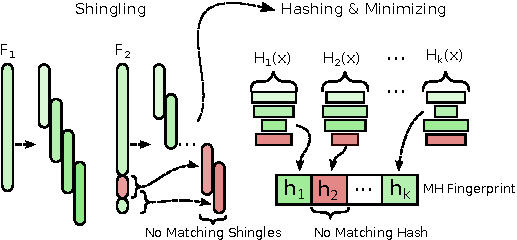
\includegraphics[scale=1]{Figures/F3M_MinHash.pdf}
\caption{The MinHash algorithm: Textual documents are broken up into overlapping shingles; Each shingle is hashed using $k$ hash functions, retaining only the smallest hash for every function, producing a fingerprint of $k$ elements. Figure taken from  \cite{F3M:FastFocusedFunctionMerging}.}\label{fig:testsvg}
\end{figure}

In the MinHash fingerprint, each hash value approximately represents a randomly selected shingle from the function. When identical sets of hash values appear in two different fingerprints, it strongly indicates that both functions contain the same instruction sequence at some point. Conversely, differing hash values suggest a reduced likelihood that the functions share that particular code pattern. This property allows MinHash to efficiently estimate the structural similarity between functions without direct instruction-by-instruction comparison.

\subsubsection{Comparing the Fingerprints}
After generating the fingerprints for the functions, each function needs to look for another function which it most likely aligns with using the fingerprints. The first step is to find a way to compare the fingerprints and quantify their similarity. This can be done by calculating the Jaccard's index between two functions' fingerprints, which is the ratio of identical pairwise hash values ($A \cup B$) to the number of hash functions ($k$):
$$J(A, B) = \frac{|A\cap B|}{k}$$

One approach is to find the best candidate function for each function by exhaustively calculating the Jaccard's index for every function and merging the candidate with the highest index score. Despite the complexity of the index calculation having been lowered from linear to constant due to the fixed size of the fingerprints, this can still be expensive.


\subsubsection{Locality Sensitive Hashing (LSH)}
F3M employs \textbf{\textit{Locality Sensitive Hashing (LSH)}} as a more efficient nearest neighbour searching approach by pruning the search space \cite{F3M:LSH}. LSH works by splitting the fingerprint vector into $b$ non-overlapping sub-vectors. Each sub-vector is hashed to produce $b$ values or \textit{bands}. When two fingerprints are similar, they will share at least one band, while dissimilar fingerprints tend not to share any bands at all. During the searching process, the nearest functions can be determined by looking at any other functions that share at least one band with the current function. This process decreases the number of functions to search through to find the most viable candidate, speeding up the search for candidate functions to merge with. This can be visualised in figure \ref{fig:F3M:LSH}

\begin{figure}[h!]
\centering
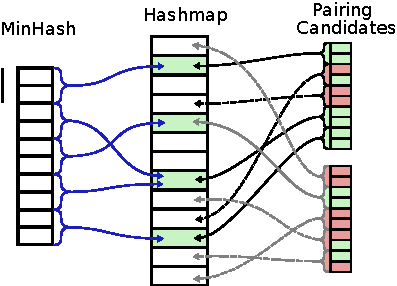
\includegraphics[scale=1]{Figures/F3M_LSH.pdf}
\caption{\textbf{Locality Sensitive Hashing} - The fingerprint on the left side represents a candidate function, and the pairing fingerprint on the right side represents potential functions to merge with the candidate. The pairing fingerprints share at least one band with the candidate fingerprint, so they will be considered during candidate lookup. Figure taken from  \cite{F3M:FastFocusedFunctionMerging}.}\label{fig:F3M:LSH}
\end{figure}

\subsubsection{Merging Functions}
Since F3M mainly focuses on improving the function selection process, it reuses the code generator used by HyFM \cite{HyFM:FunctionMergingForFree}. Code generation involves two steps: aligning instruction subsequences and generating a unified code from the alignment.

\paragraph{Instruction Alignment}
Function merging requires identifying similar instruction sequences that can be combined, and sequences that differ and require special handling. HyFM introduced, and F3M adopted, a more efficient approach by aligning at the \textbf{basic-block level} rather than function level. This significantly reduces computational overhead since basic blocks are typically much shorter than entire functions, mitigating the impact of alignment algorithms' complexity.
To align instructions, we must first define what makes instructions match. Two instructions are considered matching if they can be merged to produce a single instruction. F3M offers two complementary alignment methods with different trade-offs between speed and flexibility:

\subparagraph{Needleman-Wunsch Alignment (NW)}
For blocks with different sizes, F3M employs the NW algorithm originally introduced to function merging by FMSA \cite{FunctionMergingSequenceAlignment}. This dynamic programming approach, borrowed from bioinformatics, where it identifies similarities between protein sequences, can optimise alignments between instruction sequences of different lengths \cite{NeedlemanWunschAlgorithm}. While this NW-based approach can align instruction matches even when instructions appear at different relative positions in their respective functions, this algorithm has quadratic time and space complexity relative to the sequence length. This approach works by inserting gaps in both sequences to create equal-length sequences with optimal alignment, where matching instructions align. In contrast, non-matching instructions align with gaps, demonstrated in figure \ref{fig:SequenceAlignment2Funcs}.

\begin{figure}[tbh!]
\centering
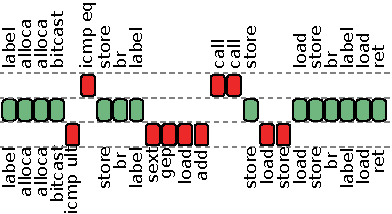
\includegraphics[scale=1]{Figures/FMSA_FunctionSA.pdf}
\caption{\textbf{Sequence Alignment between Two Functions}, green nodes represent equivalent instructions and are aligned next to each other, and red nodes represent un-equivalent instructions, placed next to the gaps. Figure taken from \cite{FunctionMergingSequenceAlignment}.}\label{fig:SequenceAlignment2Funcs}
\end{figure}

\subparagraph{Pairwise Alignment (PA)}
HyFM observed that most profitably merged basic blocks have highly similar structures \cite{HyFM:FunctionMergingForFree}. PA exploits this observation by only attempting to match instructions at corresponding positions in blocks of equal size. This strict positional alignment has linear time complexity, providing a speed-up over the NW alignment.

\subparagraph{Alignment Score} \label{METRIC:AlignmentScore}
The alignment between two functions is a property that identifies the structural similarity between two functions, serving as an early predictor of function merging profitability and is the characteristic our machine learning model aims to predict. To quantify this characteristic, the alignment score is defined as the ratio of aligned instructions to the union of aligned ($A$) and unaligned ($U$) instructions:

$$Alignment\ Score = \frac{|A|}{|A\cup U|}$$
Using figure \ref{fig:SequenceAlignment2Funcs}, we can calculate the alignment score as follows:
$$\frac{No.\ of\ Green\ Nodes}{Total\ No.\ of\ Green\ and\ Red\ Nodes}=\frac{14}{24} = 0.5833$$

Given that this metric is a ratio, this metric will be a continuous value in the range of [0, 1] inclusive, where 0 represents an entirely dissimilar function pair, and 1 represents a structurally identical function pair.

\paragraph{Code Generation From Alignment}
Once the instruction alignment is complete, F3M uses the alignment results to generate a unified function that combines the functionality of both input functions. This process follows HyFM's code generation approach. The merged functions are constructed with an additional parameter, the function identifier, which controls the original function's behaviour to execute. The code generator processes the alignment as follows:

\subparagraph{Handling Matched vs. Unmatched Code}
A single instruction is generated for matching instruction pairs that execute unconditionally in the merged function to serve both original functions. For non-matching instructions, the code generator includes them in the merged function by guarding their execution within conditional branches based on the function identifier. This ensures that the merged function preserves the exact semantics of both original functions.

\subparagraph{Control Flow Graph (CFG) Construction}
The CFG of a function represents the flow of the function, where a node corresponds to a basic block and each directed edge corresponds to a possible transfer of control (e.g. branch) between the blocks, capturing all the execution path through the function \cite{ControlFlowGraph}. The CFG of a merged function is constructed by breaking the original basic blocks into smaller ones that separate matching from non-matching code.


\section{Machine Learning} \label{Background:ML}
Machine learning (ML) offers an alternative by shifting from explicitly programmed rules to data-driven decision models. The fundamental advantage of ML-based approaches lies in their ability to discover and leverage intricate patterns across multiple code structures and behaviour dimensions.

\subsection{Supervised Learning}
Supervised learning is a machine learning paradigm in which learning is guided by labelled data \cite{MLParadigms} \cite{SupervisedLearningAndTrainingProcess}. In this approach, each input example is paired with a corresponding output, allowing the model to learn a mapping from inputs to outputs by minimising a defined loss function. This process often involves iterative optimisation techniques to adjust model parameters and improve prediction accuracy. 

In our context, supervised learning enables a model to predict the similarity of two functions by training on examples of previously merged functions and their alignment score.

\subsection{Loss Function} \label{ML:LossFunction}
A loss function is a mathematical function that quantifies the difference between the model's current predicted value and the ground truth.

Loss functions fall into two primary categories corresponding to the tasks, regression models (predicting from a continuous spectrum) and classification models (predicting from a discrete set of values). This paper will focus on regression loss functions to predict the alignment score (section \ref{METRIC:AlignmentScore}) for a pair of functions.

\subsubsection{Mean Squared Error (MSE)}
Mean squared error is a widely used loss function for regression tasks, defined by the following formula: 
$$MSE=\frac{\sum^n_{i=1}(y_i-\hat{y}_i)^2}{n}$$

\hspace{1cm} $y_i = $ Ground Truth Value

\hspace{1cm} $\hat{y}_i = $ Predicted Value

\hspace{1cm} $n = $ Number of Samples

The squaring operation in MSE provides two benefits. First, it makes all errors positive, ensuring that when multiple errors are combined and averaged in a batch, positive and negative errors do not cancel each other out. Second, it emphasises larger errors due to the quadratic nature of the function, prioritising the reduction of substantial prediction errors before fine-tuning smaller discrepancies, a desirable property when dealing with small values in the range of 0-1.

A smaller MSE is better, signifying reduced discrepancy between the predicted value and the ground truth. For our function merging application, MSE is preferable to alternatives like Mean Absolute Error (MAE) because the quadratic penalty helps the model focus on avoiding large prediction errors that could lead to poor merging decisions.

\subsection{Gradient Descent} \label{ML:Gradients}
Gradient descent, the primary optimisation algorithm in deep learning, uses forward and backward propagation. During \textbf{forward propagation}, the model processes the training data through itself to produce a set of predictions. The loss function quantifies the error between these predictions and the ground truth.

During \textbf{backward propagation}, the gradient for the loss function is calculated with respect to each parameter in the model using the chain rule. The gradients indicate the direction and magnitude of parameter adjustment needed to reduce the loss \cite{GradientDescentBackpropagation1, GradientDescentBackPropagation2}.

Using this information, gradient descent adjusts each parameter in the opposite direction of the gradient, scaled by the selected learning rate \cite{DeepLearningGoodfellow}. This process iteratively navigates the parameter space toward a local minima of the loss function if it is well designed. Finding a global minima is not always possible, so a well-suited local minima is sufficient for predictions.

All gradient descent methods aim to minimise the loss function, iteratively refining the model to make predictions that more closely match the ground truth.

\subsection{Hyperparameters}
An ML model usually has hyperparameters to configure. These model parameters are not learnt and configured before a model starts training. Unlike model weights, which are optimised during training, hyperparameters control the learning process itself. They control how the model learns and behaves from the input data. A subset of the dataset, the validation set, is usually set aside to tune the hyperparameters. Some of the most common hyperparameters are discussed below.

\paragraph{Epochs} \label{ML:Epochs} The number of epochs specifies the number of times the model trains using the entire training data. Setting a value that is too low may cause the model to underfit\footnote{\textbf{Underfitting} - When a model is unable to capture the underlying patterns in the training data, leading to poor performance on training and unseen data} to the training data, while a value that is too high may cause the model to overfit\footnote{\textbf{Overfitting} - When a model starts memorising the training data, capturing noise and irrelevant information instead of trying to learn the patterns associated with the data leading to poor generalisation on unseen data} to the training data, causing a drop in performance when evaluated against the validation set. One way to prevent this type of overfitting is by implementing early stopping. Early stopping monitors the model's performance on the validation data, halting training when the validation performance degrades, preventing overfitting.

\paragraph{Learning Rate} \label{ML:LearningRate} The learning rate determines the size of the step taken by the model for each training iteration, a large learning rate would magnify the loss function more than a smaller learning rate. Selecting a large value means less time is needed for training, but the model may overshoot the global minimum and struggle to converge. On the other hand, if the learning rate is too small, the model will converge on a local minimum and be unable to leave it, thus not finding the optimal solution \cite{LearningRate}. Adaptive learning rate techniques like Adam can adjust the learning rate dynamically during training to improve convergence \cite{GradientDescentAlgorithms}.


\paragraph{Batch Size} \label{ML:BatchSize} The batch size specifies the number of training samples processed in each training iteration. The loss and gradient are averaged for all training samples in a batch. Selecting a suitable batch size is important. One too small produces noisy gradient estimates, leading to unstable weight updates, hampering convergence toward the true minimum. At the same time, one that's too large requires more memory and may smooth over important gradient details, potentially causing convergence to a suboptimal solution \cite{BatchSizeTooLarge, BatchSizeVariance, DeepLearningGoodfellow}.


\paragraph{Hyperparameter Optimisation} Hyperparameter optimisation is fundamentally an iterative process of proposing hyperparameter settings, training the model and evaluating its performance on a validation dataset. The hyperparameter settings are refined until the optimal validation performance is reached. \textbf{Grid search} exhaustively samples this space but becomes inefficient as the dimensionality grows \cite{BayesianFasterThanGrid}. \textbf{Bayesian optimisation} is an alternative which builds a probabilistic model of the model's performance on the validation set to suggest promising hyperparameters effectively \cite{BayesOptimisationOriginal}. At each step, Bayesian optimisation maintains a belief about how well different hyperparameter settings will perform, then uses the results of past trials to update that belief using Bayes Theorem \cite{BayesTheorem}. This updated belief is used to influence the following settings to try, balancing the desire to explore uncertain regions against the chance of finding an even better result. In this way, Bayesian optimisation focuses effort where it is most likely to pay off, often finding high-performance configurations in fewer trials than grid search \cite{BayesianFasterThanGrid}.

\subsection{Imbalanced Dataset}
In a perfect world, a dataset will have a similar amount of data samples across the output data's range/spectrum, but this is not always possible. If no effort is taken to take into account the imbalance of the data samples, a model will learn to predict more of the dominant data samples. To mitigate this, sample weightings can be used, which will scale down the loss for the dominant data points and scale up the loss for under-represented data points. This is known as \textbf{cost-sensitive learning (weighting)} \cite{ImbalancedDataset}. This ensures that the loss function will reasonably adjust the parameter without overfitting itself to predict more for the dominant data points.

% \subsection{Testing}
% Finally, another third subset of the dataset is set aside to evaluate the model's overall performance, known as the testing set. It is crucial that this set of data has not been used or seen at all by the model, so that the model's final evaluation can be unbiased on its ability to generalise to unseen data. The subsets of data that have been discussed so far, training, validation and testing should all be divided up at the start before model training to prevent data from training to be used for evaluation or vice versa. For regression tasks, mean-squared error (MSE), mean absolute error (MAE) and mean absolute percentage error (MAPE) are popular options. The MSE was selected as the metric because it emphasises larger errors, especially important when we are dealing with such small numbers and the MAPE is unable to deal with ground truth values that are 0 as division with 0 is not possible.

\subsection{Other Applications of ML in compilers}

% \subsubsection{Optimisation Selection}
% Optimisation selection determines which compiler optimisations should be applied to a program to achieve the best performance, code size, or other objectives. Compilers typically have dozens or hundreds of individual optimisation passes available, each with various parameters and settings. \todo{CITE Optimisation SELECTION}

% The challenge lies in deciding which optimisations to apply to a particular program, in what order, and with what parameters. Traditionally, compilers use predefined heuristics based on fixed rules established by compiler developers. However, these heuristics often fail to capture the complex interactions between optimisations and program characteristics across different architectures.

% Optimisation selection using machine learning has emerged as a powerful approach to automate compiler optimisations. MILEPOST GCC represents one of the pioneering efforts in this area, automatically adjusting compiler optimisation heuristics to improve execution time, code size, or compilation time \cite{OptimisationSelectionML}. The system collects program features and execution feedback and then uses this data to train models that predict optimisation strategies for new programs. This approach eliminates the need for expert hand-tuning of optimisation heuristics for each new architecture or program. Experimental results showed that MILEPOST GCC could reduce the execution time of the MiBench benchmark suite on the ARC processor architecture.

% The key innovation of this approach is that it replaces static, hardwired compiler optimisation decisions with data-driven models that can adapt to different architecture characteristics. This makes porting optimisation compilers to new hardware significantly more efficient, as the system automatically learns appropriate optimisation strategies rather than requiring manual recalibration.

% \subsubsection{Iterative Compilations}
% Iterative compilation is a technique that repeatedly compiles a program with different optimisation settings and evaluates the resulting performance to find the best configuration. Rather than relying on heuristics to determine the optimal optimisation strategy upfront, iterative compilation empirically explores the space of possible optimisations. \todo{CITE ITERATIVE COMPILATION}
% Iterative compilation traditionally requires extensive and repetitive fine-tuning to find optimal compiler optimisations, which creates a significant bottleneck in the development process. This challenge is addressed by applying active learning techniques to minimise the cost of iterative compilation \cite{IterativeCompilationWActiveLearningML}.
% The research demonstrated that traditional iterative compilation wastes substantial effort collecting redundant training data. Many of the performance measurements collected contribute little to the final optimisation heuristic. Their approach optimised both the selection of training examples and the number of samples per example using sequential analysis.

% By applying active learning principles, their methodology reduced training overhead compared to approaches with fixed sampling plans. The system determines dynamically whether additional samples are needed for a particular configuration based on the current model's uncertainty. This transforms what would typically take months of compilation and performance measurements into days, making machine learning-based compilation much more practical for real-world deployment.

% \subsubsection{Loop Vectorisation}
% Loop vectorisation is a compiler optimisation technique that transforms sequential loop operations to take advantage of modern processors' SIMD (Single Instruction, Multiple Data) capabilities. Instead of processing one data element per instruction, vectorisation allows a single instruction to simultaneously operate on multiple data elements. \todo{CITE LOOP VECTORISATION}

% Loop vectorisation is a critical compiler optimisation for modern SIMD-compatible architectures. NeuroVectorizer represents a significant advance in this area by using deep reinforcement learning to predict optimal vectorisation factors for loops \cite{LoopVectorisationML}.

% Traditional vectorisers in compilers like LLVM use fixed-cost models based on heuristics to make vectorisation decisions. These models struggle to accurately capture data dependencies, computation graphs, and instruction organisations. NeuroVectorizer takes a fundamentally different approach by employing a neural network that learns code embeddings directly from loop source code and then uses reinforcement learning to determine the optimal vectorisation and interleaving factors.

% The system achieved impressive results, showing performance speedup compared to the baseline LLVM vectoriser across various benchmarks. The reinforcement learning model proved particularly effective because it can learn complex patterns from code structure without requiring explicit feature engineering and can co-optimise multiple objectives like execution time and code size simultaneously.

% \subsubsection{Function Inlining}
% Function inlining is a compiler optimisation that replaces a function call with the called function's actual body. This eliminates the overhead of the function call mechanism (saving the registers, jumping to the function code, returning, and more) \todo{CITE Function Inlining}. MLGOPerf extends machine learning approaches to function inlining decisions in LLVM \cite{FunctionInliningML}.

% While MLGO (Machine Learning Guided Optimisation) previously focused on optimising code size with ML-based inlining, MLGOPerf specifically targets performance optimisation. The system employs two ML models: a primary reinforcement learning model that makes inlining decisions and a secondary model (IR2Perf) that predicts post-inlining speedup to generate rewards for training the RL agent.
% This two-model approach enables fast training without requiring the time-consuming execution of actual programs for each training iteration. Experimental results showed that MLGOPerf improved performance over LLVM's O3 optimisation level on SPEC CPU2006 and Cbench benchmarks. 
% Function inlining optimisation represents a particularly challenging problem due to the exponential growth of the optimisation space, making machine learning approaches especially valuable in this domain.

\paragraph{Optimisation Selection} Optimisation Selection focuses on determining which compiler optimisations to apply to a program to enhance performance, reduce code size, or meet other objectives. Traditionally, compilers have relied on fixed rule-based heuristics developed by compiler engineers to choose from a vast array of optimisation passes. However, with techniques like those used in MILEPOST GCC, machine learning models now collect program features and runtime feedback to automatically predict the most beneficial optimisation strategies, thereby replacing static rules with adaptable, data-driven decisions \cite{OptimisationSelectionML}.

\paragraph{Iterative Compilation} Iterative Compilation tackles the optimisation challenge by repeatedly compiling a program with different settings and empirically testing the resulting performance. Instead of depending solely on predefined heuristics, this method explores a broader range of optimisation configurations to identify the optimal solution. The process is enhanced by active learning strategies which intelligently select training examples and adjust sampling dynamically based on the model's uncertainty. This adaptive approach dramatically reduces the time and effort required for extensive fine-tuning \cite{IterativeCompilationWActiveLearningML}.

\paragraph{Loop Vectorisation} Loop Vectorisation is a compiler optimisation that transforms sequential loop operations to exploit the parallel processing capabilities of SIMD hardware. Traditional vectorisers use fixed-cost heuristic models that may not fully capture the complex data dependencies and instruction patterns within code loops. In contrast, advanced approaches like NeuroVectorizer use deep reinforcement learning to predict the best vectorisation factors for loops. This method learns code representations directly from the source code, allowing it to determine more effective vectorisation and interleaving factors \cite{LoopVectorisationML}.

\paragraph{Function Inlining} Function Inlining is a technique that replaces a function call with the body of the function itself, thereby eliminating the overhead associated with calling a function. Recent advances, such as MLGOPerf, extend machine learning techniques to optimise inlining decisions. This approach leverages a two-model strategy: a primary reinforcement learning model for decision making and a secondary model to predict the performance gains from inlining. By doing so, the system efficiently optimises inlining, and has demonstrated improvements in performance on standard benchmarks compared to traditional inlining strategies \cite{FunctionInliningML}.

\section{Neural Networks} \label{Background:NeuralNetworks}
Neural networks are powerful machine learning models inspired by the structure and function of the human brain. They automatically learn hierarchical representations from raw inputs through \textbf{artificial neurons} arranged in an input layer, hidden layers, and an output layer. Each neuron receives input signals, applies weights and biases, and passes the result through a non-linear activation function to produce an output. A network's performance is influenced by its \textbf{depth} (number of layers) and \textbf{width} (neurons per layer). Training involves optimisation algorithms like gradient descent and back-propagation to adjust weights and minimise a loss function.

\subsection{Semantical Representations} \label{subsection:SemanticalRepresentations}
% Machine learning models face a fundamental limitation when processing data, they operate exclusively on numerical values. This creates a significant challenge when working with symbolic or textual data, such as program code. Since these algorithms rely on mathematical operations, inputs must be represented numerically; raw non-numeric data cannot be directly processed or learnt from.

% To overcome this limitation, the inputs should be transformed into a numerical representation that preserves semantic relationships and enables effective machine learning. Word embeddings are a prime example of this transformation, as they map words into dense, continuous vector spaces that capture semantic information.

% Simple encoding techniques like \textbf{one-hot encoding}, where each unique symbol is assigned its own dimension in a vector space, fail to capture meaningful relationships between elements because all symbols are equidistant, so the encoding does not reflect any inherent similarity or dissimilarity between words. Moreover, as vocabulary size increases, one-hot encoding leads to extremely high-dimensional and sparse representations. This results in inefficient use of memory and significantly increases the computational cost of training machine learning models \cite{DeepLearningGoodfellow}.

% For instance, \textbf{word2vec} employs a shallow neural network with two primary architectures, the \textit{Continuous Bag-of-Words (CBOW)} model and the \textit{Skip-Gram} model \cite{Word2Vec}. In the CBOW approach, the network predicts a target word based on its surrounding context words, while the Skip-Gram model does the inverse by predicting context words given a target word. Both models learn embeddings by optimising the prediction task over a large corpus, ensuring that semantically similar words are located near each other in the resulting vector space. Similarly,  \textbf{GloVe}  was proposed as a method that leverages global word co-occurrence statistics to generate embeddings reflecting nuanced linguistic relationships \cite{GloVe}.

% These embedding techniques enable machine learning models to effectively utilise the underlying semantics of the symbolic data to predict future tasks.


Machine learning models face a fundamental limitation when processing data, they operate exclusively on numerical values. This creates a significant challenge when working with symbolic or textual data, such as program code. Since these algorithms rely on mathematical operations, inputs must be represented numerically.

To overcome this limitation, inputs should be transformed into numerical representations that preserve semantic relationships. Word embeddings exemplify this approach by mapping words into dense, continuous vector spaces that capture semantic information.

Simple encoding techniques like \textbf{one-hot encoding} fail to capture meaningful relationships between elements because all symbols are equidistant, resulting in inefficient high-dimensional, sparse representations that increase computational costs.

More advanced embedding techniques (word2vec and GloVe) enable machine learning models to effectively utilise the underlying semantics of symbolic data for prediction tasks \cite{Word2Vec, GloVe}.

\subsubsection{IR2Vec} \label{subsubsec:IR2Vec}
% IR2Vec is a framework that generates embeddings for LLVM's Intermediate Representation (LLVM IR) \cite{IR2Vec}. Unlike traditional word embeddings that map natural language tokens into dense vector spaces, IR2Vec transforms programs and functions into vector representations by modelling the relationships among IR entities, such as opcodes, types, and operands, using a translational embedding model, like \textit{TransE} \cite{TranslationalEncoding}.

% This process begins by extracting relational information from the LLVM IR, which IR2Vec stores as a triplet ($<h, r, t>$). $h$ (head) represents an entity in the IR, $t$ (tail) represents another entity in the IR that has a relationship with $h$, and $r$ (relation) represents the relationship between $h$ and $t$. The triplets are then processed using a translation-based embedding model inspired by \textit{TransE}. The core idea of \textit{TransE} is that relationships should be represented by vectors such that the sum of the relation vector $r$ with the head vector $h$ should approximate the tail's vector $t$.
% $$h+r\approx t$$

% Relying on this concept, IR2Vec can build up the vector representations of the fundamental components of the IR (opcodes, operands, ...) known as \textbf{seed encoding}. These seed embeddings can then be used to build up higher-level embeddings for higher-level program abstraction like instructions, basic blocks, functions and modules, referred to as \textit{Symbolic Encoding}.

% IR2Vec offers an even richer embedding by incorporating the program's flow details, like the use-def chains and the reaching definitions, into the symbolic encoding, aptly named \textit{flow-aware encoding}. This allows the encoder to capture the program's operational semantics in addition to the syntactical information, facilitating more effective analyses and optimisations. 

% IR2Vec is fully open-source, facilitating straightforward customisation and extension. It is available across multiple platforms, it can be utilised as a Python library, a C++ library, or even as a stand-alone binary, ensuring seamless integration into various development environments.

IR2Vec is a framework that generates embeddings for LLVM's Intermediate Representation (LLVM IR) \cite{IR2Vec}. Unlike traditional word embeddings, IR2Vec transforms programs and functions into vector representations by modelling the relationships among IR entities, such as opcodes, types, and operands, using a translational embedding model like \textit{TransE} \cite{TranslationalEncoding}.

The process extracts relational information from LLVM IR as triplets (<h, r, t>), representing relationships between entities. Using these triplets, IR2Vec builds vector representations of the IR's fundamental components (opcodes, operands, etc.) as seed encoding. These seed embeddings then construct higher-level embeddings for instructions, basic blocks, functions and modules (Symbolic Encoding).

IR2Vec offers an even richer embedding by incorporating the program's flow details, like use-def chains and reaching definitions, into the symbolic encoding (flow-aware encoding), capturing both operational semantics and syntactical information for more effective analyses and optimisations.

IR2Vec is fully open-source, facilitating straightforward customisation and extension. It is available across multiple platforms, it can be utilised as a Python library, a C++ library, or even as a stand-alone binary, ensuring seamless integration into various development environments.

\subsection{Activation Functions}
Activation functions are mathematical operations applied to the output of neural network layers that introduce non-linearity, allowing networks to learn complex patterns beyond what linear combinations can express. The ReLU (Rectified Linear Unit) activation function has become the standard choice for hidden layers, outputs a value in the range $[0, \infty )$, passing through positive inputs unchanged while zeroing out negative values. In contrast, the Sigmoid activation function squashes inputs to outputs between 0 and 1, making it well-suited for models that need values to be normalised within a bounded range. Figure \ref{fig:SigmoidReluGraph} shows the graphs of the sigmoid and ReLU activation functions.

\begin{figure}[h!]
\centering
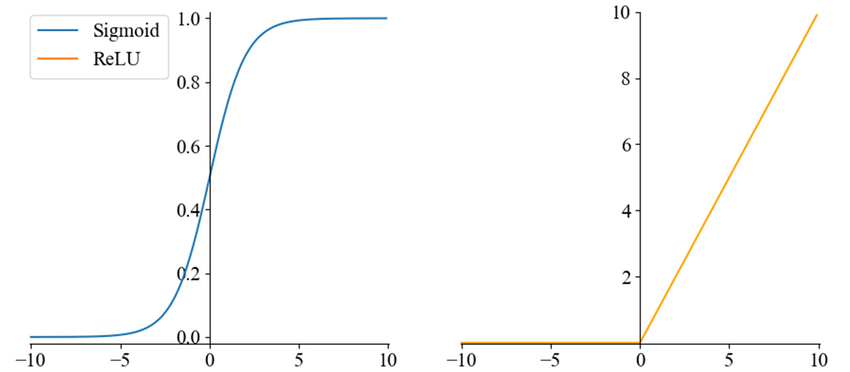
\includegraphics[scale=0.45]{Figures/SigmoidRELUActivationFunction.png}
\caption{Graph of sigmoid activation function on the left and the ReLU activation on the right. Figure taken from  \cite{SIgmoidRELUGraph}.}\label{fig:SigmoidReluGraph}
\end{figure}


\subsection{Layers}
This section will discuss the layers and techniques used in the paper.
\subsubsection{Dense Layers}
Dense or fully connected layers are a fundamental building block of neural networks. In a dense layer, every artificial neuron is connected to every neuron in the preceding layer, creating a network of weighted connections \cite{DeepLearningGoodfellow}. The number of neurons in a dense layer could also be treated as a hyperparameter to be tuned. A dense layer performs the following mathematical transformation: 
$$y = \sigma(Wx+b)$$

\hspace{1cm}$x = $ Input vector from the previous layer

\hspace{1cm}$W = $ Weights matrix

\hspace{1cm}$b = $ Bias vector

\hspace{1cm}$\sigma =$ An activation function to introduce non-linearity

Dense layers are known for their powerful feature extraction abilities by learning complex patterns and relationships within data. They transform an input's representation into a more abstract representation. The primary advantages of dense layers include their flexibility in handling fixed-size vector inputs and their strong representational capacity. 

This layer can lead to overfitting in deep learning networks, which is why dense layers are often used with regularisation techniques.

\subsubsection{Dropout Layer}
Regularisation techniques seek to prevent overfitting by introducing controlled noise during training so that models learn representations that generalise beyond the training set. One of the most popular methods for neural networks is dropout, which directly alters the network's architecture during training instead of the usual modification of the loss function. 

At its core, dropout is very simple, each neuron in a layer is randomly deactivated on each training sample with probability $p$ (dropout rate). Equivalently, each neuron is kept with probability $q=1-p$. During the forward pass, a binary mask $m$ of independent Bernoulli random variables is sampled and applied to the neurons, any surviving neurons are scaled by $\frac{1}{1-p}$ so that their expected value remains unchanged \cite{DropoutPaper}.

Normal neural layer's mathematical representation:
$$y = f(Wx + b)$$
After applying dropout:
$$y=f(Wx+b)\times \textbf{m}$$
There are two variants of dropout, the standard dropout which applies the scaling during inference, and the inverted dropout which applies the scaling during training. Modern frameworks use inverted dropout by default to simplify inference \cite{TensorflowDropout, PyTorchDropout}.

Typical choices for the dropout rate $p$ range from 0.2 to 0.5, although these values should be treated as hyperparameters and tuned for each task \cite{DropoutPaper}.

\subsubsection{Multi-Headed Attention Layers} \label{ML:AttentionMechanism}
Attention layers allow a neural network to focus on the most important feature of the current task. Not all parts of the input contribute equally to solving a problem; by learning which elements require more attention, the network can make more informed decisions. 

The attention mechanism takes in two inputs, the first input will attend to the second. There are two variants of attentions, \textbf{self-attention} where both inputs are the same, so the sequence is attending to itself, or \textbf{cross-attention} where both inputs are different.

The attention mechanism starts with three learned weights used to create three vectors from the inputs, the query (Q) vector is created from the first input, and the key (K) and value (V) vectors are created from the second input. 

Then, it compares each query against all available keys to find how well each key matches the query by calculating the dot product of the pair. High-scoring pairs are given more attention while low-scoring pairs are given less attention or ignored. The scores are then put through a softmax function that converts each score into a probability. Then, the value vector is multiplied by the weight, and the elements are summed up to generate a weighted sum to produce the first input's new vector representation after attending to the second input \cite{AttentionIsAllYouNeed}.

The model then uses the newly attended vector for further processing and prediction. The error is calculated, and backpropagation is then used to update the weights to generate the Q, K and V vectors.

A multi-headed attention layer takes it one step further by having multiple attention layers in parallel to model different relationship aspects. This works by dividing the Q, K and V vector representations across the number of parallel attention mechanisms, each mechanism is known as a head. Each head works on its allocated portion of the Q, K and V values before being concatenated to form the final representation, which is typically projected back to the original dimension.

Despite its effectiveness, attention and multi-headed attention models come with higher computation costs than traditional mechanisms due to the attention mechanism's nature, where every element in the sequence must attend to every other element, resulting in a $O(n^2)$ complexity with respect to the input length \cite{AttentionComplexity}.



\subsection{Siamese Neural Network} \label{ML:SiameseNetwork}
Siamese neural networks are a class of artificial neural networks that process two inputs in parallel using identical sub-networks with shared weights to produce comparable output embeddings. The embeddings are then compared using a distance or similarity function to produce a value suitable for verification and matching tasks \cite{SiameseModelIntro}.

The architecture's key characteristic is the weight-sharing constraint between sub-networks, which ensures that similar inputs are mapped to nearby points in the embedding space while dissimilar inputs are mapped to distant points. Additionally, this ensures that the embedding is consistent across both inputs, enabling the model to generalise similarity judgements on unseen pairs.

Siamese networks have found wide applications in signature verification, face recognition, and image similarity assessment \cite{SiameseModelSignatureVerification, SiameseFacialRecognition, SiameseImageSimilarity}. Their effectiveness stems from learning a discriminative embedding space rather than direct classification.

Numerous metrics can be employed to measure the similarity between embeddings. In this paper, we focus on the following three:

\paragraph{Manhattan Distance}
The Manhattan distance, also known as the L1 distance, measures similarity by computing the sum of absolute differences between corresponding elements of two vectors, increasing with dissimilarity. For embeddings $a$ and $b$ of dimension $n$, the distance is calculated as:

$$d(a, b) = \sum^n_{i=1}|a_i - b_i|$$


\paragraph{Dot Product} \label{METRIC:DotProduct}
The dot product, also known as the inner product between two vectors $a$ and $b$, is computed as:

$$\sum^n_{i=1}a_i \times b_i$$

When used as a similarity metric in Siamese networks, the dot product measures the directional alignment and magnitude correlation between embeddings. A higher dot product indicates a higher similarity. 

\paragraph{Cosine Similarity} \label{METRIC:CosineDistance}
Cosine similarity is the cosine of the angle between two vectors. It is defined as the normalised dot product of the vectors, removing the influence of vector magnitude and focusing only on the directional similarity. For embeddings $a$ and $b$, cosine similarity is calculated as:

$$cos(\theta) = \frac{a.b}{|a||b|}$$

The result ranges from $-1$ to $1$, where $-1$ indicates vectors pointing exactly opposite directions, $0$ represents orthogonal vectors with no directional correlation, and $1$ signifies vectors pointing in the same direction. 